\section{Canonical}
\label{sec:canonical}

\par Canonical is the company that launched Ubuntu project in 2004. Founded by South African \href{http://www.markshuttleworth.com/}{Mark Shuttleworth} after a profit of 500\$ million from the sale of his  security company. \href{http://www.markshuttleworth.com/archives/4}{Decided to invest} the money to create a Linux distribution more friendly and easy to install

\begin{quote}
    \textit{"Linux for human beings"}
\end{quote}

\par So, he got in touch with \href{http://www.debian.org/index.html}{Debian} developers (which is one of the most reliable Linux distributions) to offer financial support to create a more human Linux \textit{Ubuntu}.

\par After a  controversial year because of this distribution is owned by one person, decided to create a Foundation in 2005: Ubuntu Foundation to prevent Ubuntu depended on a person or organization and was now to be directed by people. That gave decision making to community and Copyright Holder of Ubuntu to the Foundation to avoid possible distribution privatizations by a Company or a person.

\subsection{Technologies}

\par Canonical is not a software solution is a company that develops FLOSS project Ubuntu and other solutions that are not FLOSS.

\par We can take a look to Technologies used to develop Ubuntu with the community. Explained in their \href{https://wiki.ubuntu.com/}{Wiki} we summarize main goals in Get involved section and focusing our summary in Kernel development Team:

\begin{itemize}
	\item \textit{Communications}
    \begin{itemize}
	    \item \textit{Blogs} - Here is a planet that unifies all development team personal /technical blogs in one feed releated to huma project members in http://voices.canonical.com/kernelteam/.
	    \item \textit{IRC} channel \#ubuntu-kernel to get in touch with users and developers. Weekly IRC  public meeting in \#ubuntu-meeting to strengthen collaboration within the project.
	    \item \textit{Mailing List} - Mailing lists are highly used in Ubuntu, you can subscribe to contribute \href{https://lists.ubuntu.com/mailman/listinfo/kernel-team}{here}.
	    \item We run our mailing list much like the Linux Kernel Mailing List (LKML). Users can propose patches, ask questions and find general info. This list has medium traffic volume. For more info you can read https://wiki.ubuntu.com/KernelTeam/KernelPatches
    \end{itemize}
	\item \textit{Launchpad Teams} - ALM Tools from Ubuntu to deploy projects, I/BTS (Issue/Bugs Tracking System) and public roadmap.
\begin{itemize}
	\item \href{https://launchpad.net/~ubuntu-kernel-team}{Ubuntu Kernel Team} this is the moderated public team in which we interact with the Ubuntu Community.
	\item \href{https://launchpad.net/~canonical-kernel-team}{Canonical Kernel Team} this is a private team used by the Canonical Kernel Team for Canonical paid hardware enablement and other Canonical business.
\end{itemize}
	\item \textit{Contacts} - This section is special because translates developers to humans to get in touch with them, is based on the philosophy.
\end{itemize}

\subsection{How to Contribute}

\par \href{https://wiki.ubuntu.com/UbuntuDevelopment}{Ubuntu Development} describes a guide of how to contribute, collaborate and communicate in team projects. Ubuntu describes a community \href{http://www.ubuntu.com/project/about-ubuntu/conduct}{Code of Conduct}. A must read document that explains relations inside Ubuntu community, respect, responsible, collaborate, teamwork, meritocracy, ask for help. All rules to guide a respectful community teamwork based in communication and consensus. You \textbf{have to sign this contract} to contribute to Ubuntu community.

\par Encourages you to subscribe to mailing lists and start reading information about the community and how work internally.

\par After that take a look to bug section managed by \href{https://wiki.ubuntu.com/BugSquad}{BugSquads}. Here you can contribute searching and reporting bugs by your own or join a bug team specialized in a module. Bug Squad has a guide of their job described to triaging:

\begin{itemize}
	\item Responding to new bugs as they are filed.
	\item Ensuring that new bugs have all the necessary information.
	\item Assigning bugs to the proper package.
	\item Confirming bug reports by trying to reproduce them.
	\item Setting the importance of bugs reports. (Bug Control members Only)
	\item Searching for and marking duplicates in the bug tracking system.
	\item Sending bugs to their upstream authors, when applicable.
	\item Cross-referencing bugs from other distributions.
	\item Expiring old bugs.
\end{itemize} This section is very interesting because they are like bug soldiers inside a QA \textit{users} team and have a clear and strict workflow to deal with bugs.

\par \href{http://uds.ubuntu.com/}{Ubuntu Developer Summit} is an open-innovation section:

\begin{quote}
    \par \textit{"The bulk of UDS is discussion sessions. We explore problems and develop solutions together, pooling our collective experience"}
\end{quote}

\par Includes developers, proposals, technical users through the common idea to unify roads and problems, to create a team, nearly through the exchange of ideas and views. A good proposal for collaboration in the community.

\begin{figure}
  \caption{Ubuntu community organization, Antonio Carmona}
    \centering
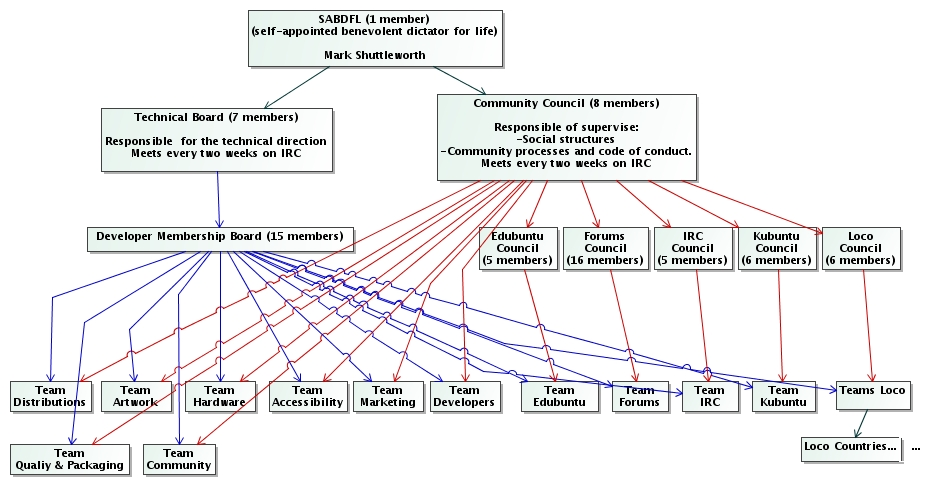
\includegraphics[width=\textwidth]{../images/MSWL-CSII-UbuntuCommunityRicardo-ACarmona.jpg}
\end{figure}

% section canonical (end)
